\subsection{Angle Bisectors}

\begin{figure}[!ht]
	\begin{center}
		
		%
\includegraphics[width=\columnwidth]{./figs/ch3_angle_bisector}
		%\vspace*{-10cm}
		\resizebox{\columnwidth}{!}{\begin{tikzpicture}
[scale=2,>=stealth,point/.style={draw,circle,fill = black,inner sep=0.5pt},]

\node (D) at (0, 0)[point,label=below :$D$] {};
\node (A) at (0, 3)[point,label=above :$A$]{};
\node (B) at (-3, 0)[point,label=below left:$B$]{};
\node (C) at (3, 0)[point,label=below right:$C$]{};
\node (O) at (0, 1.3)[point,label=below right:$O$]{};
\node (F) at (-1.1, 1.9)[point,label=above left:$F$]{};
\node (E) at (1.1, 1.9)[point,label=above right:$E$]{};

\draw (D)--(B);
\draw (B)--(A);
\draw (A)--(C);
\draw (C)--(D);
\draw [thick,dashed] (A) -- (D);
\draw [thick,dashed] (O) -- (E);
\draw [thick,dashed] (O) -- (F);
\draw (B)--(O);
\draw (C)--(O);

\tkzMarkRightAngle[size=.2](A,D,C)
\tkzMarkRightAngle[size=.15](B,F,O);
\tkzMarkRightAngle[size=.15](C,E,O);
\tkzMarkAngle[size=.4](D,B,O);
\tkzMarkAngle[size=.35](O,B,F);
\tkzMarkAngle[size=.54](E,C,O);
\tkzMarkAngle[size=.5](E,C,O);
\tkzMarkAngle[size=.6](O,C,D);
\tkzMarkAngle[size=.65](O,C,D);

\end{tikzpicture}}
	\end{center}
	\caption{Angle bisectors meet at a point}
	\label{ch3_angle_bisector}	
\end{figure}

\begin{definition}
	In Fig. \ref{ch3_angle_bisector}, $OB$ divides the  $\angle B$ into half, i.e.\begin{equation}
	\angle OBC = \angle OBA
	\end{equation}
	$OB$ is known as an angle bisector.
\end{definition}
	$OB$ and $OC$ are angle bisectors of angles $B$ and $C$. $OA$ is joined and $OD, OF$ and $OE$ are perpendiculars to sides $a,b$ and $c$.
\begin{problem}
  Show that $OD = OE = OF$.
\end{problem}
\proof In $\Delta$s $ODC$ and $OEC$,
\begin{align}
OD &= OC \sin \frac{C}{2}
\\
OE &= OC \sin \frac{C}{2} 
\\
\Rightarrow OD &=OE.
\end{align}
Similarly,
\begin{equation}
OD = OF.
\end{equation}
%
\begin{problem}
	Show that OA is the angle bisector of $\angle A$
\end{problem}
\proof In $\Delta$s $OFA$ and $OEA$,
\begin{align}
OF &= OE
\\
\Rightarrow OA \sin OAF &= OA \sin OAE \\
\Rightarrow \sin OAF &=  \sin OAE \\
\Rightarrow \angle OAF &= \angle OAE
\end{align}
which proves that $OA$ bisects $\angle A$.
{\em Conclusion:} The angle bisectors of a triangle meet at a point.


\subsection{Congruent Triangles}
%
\begin{problem}
	Show that in $\Delta$s $ODC$ and $OEC$, corresponding sides and angles are equal.
\end{problem}
\begin{definition}
	Note that    $\Delta$s $ODC$ and $OEC$ are known as congruent triangles.  To show that two triangles are congruent, it is sufficient to show that some angles and sides are equal.
\end{definition}
\begin{problem}
SSS:	Show that if the corresponding sides of three triangles are equal, the triangles are congruent.
\end{problem}
\begin{problem}
ASA:	Show that if two angles and any one side  are equal in corresponding triangles, the triangles are congruent.
\end{problem}
\begin{problem}
SAS:	Show that if two sides and the angle between them are equal in corresponding triangles, the triangles are congruent.
\end{problem}
\begin{problem}
RHS:	For two right angled triangles, if the hypotenuse and one of the sides are equal, show that the triangles are congruent.
\end{problem}
	%
%%
\subsection{Perpendicular Bisectors}
\begin{definition}
	In Fig. \ref{ch3_perp_bisector}, OD $\perp BC$ and $BD=DC$. $OD$ is defined as the perpendicular bisector of $BC$.
\end{definition}

\begin{problem}
	In Fig. \ref{ch3_perp_bisector}, show that $OA=OB=OC$.
\end{problem}
%%
%%
\begin{figure}[!ht]
	\begin{center}
		
		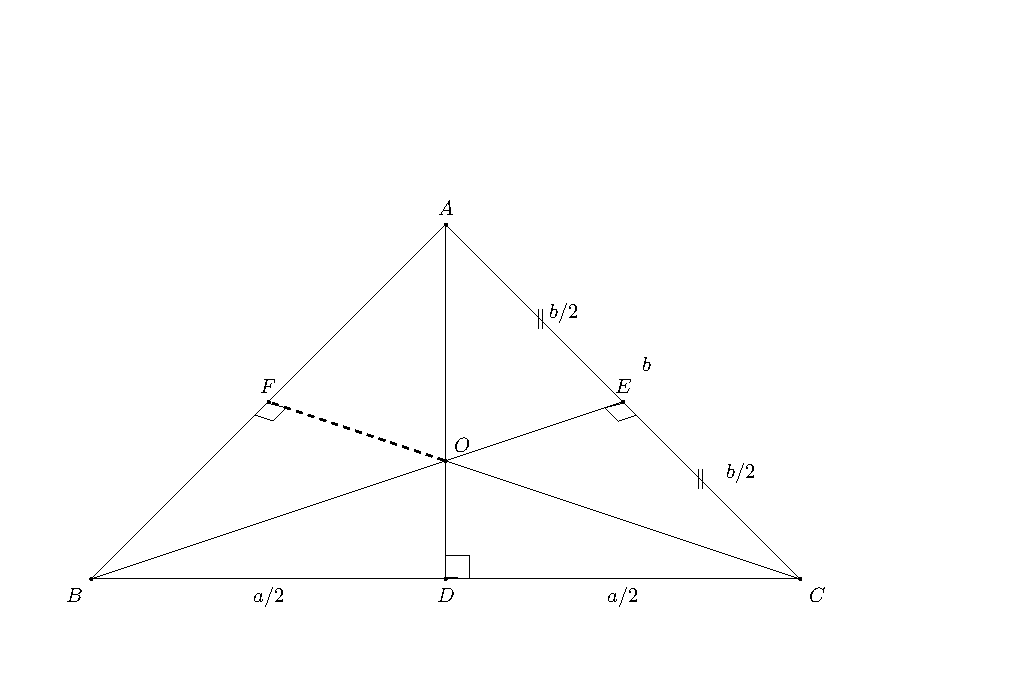
\includegraphics[width=\columnwidth]{./figs/fig_3.8.eps}
%		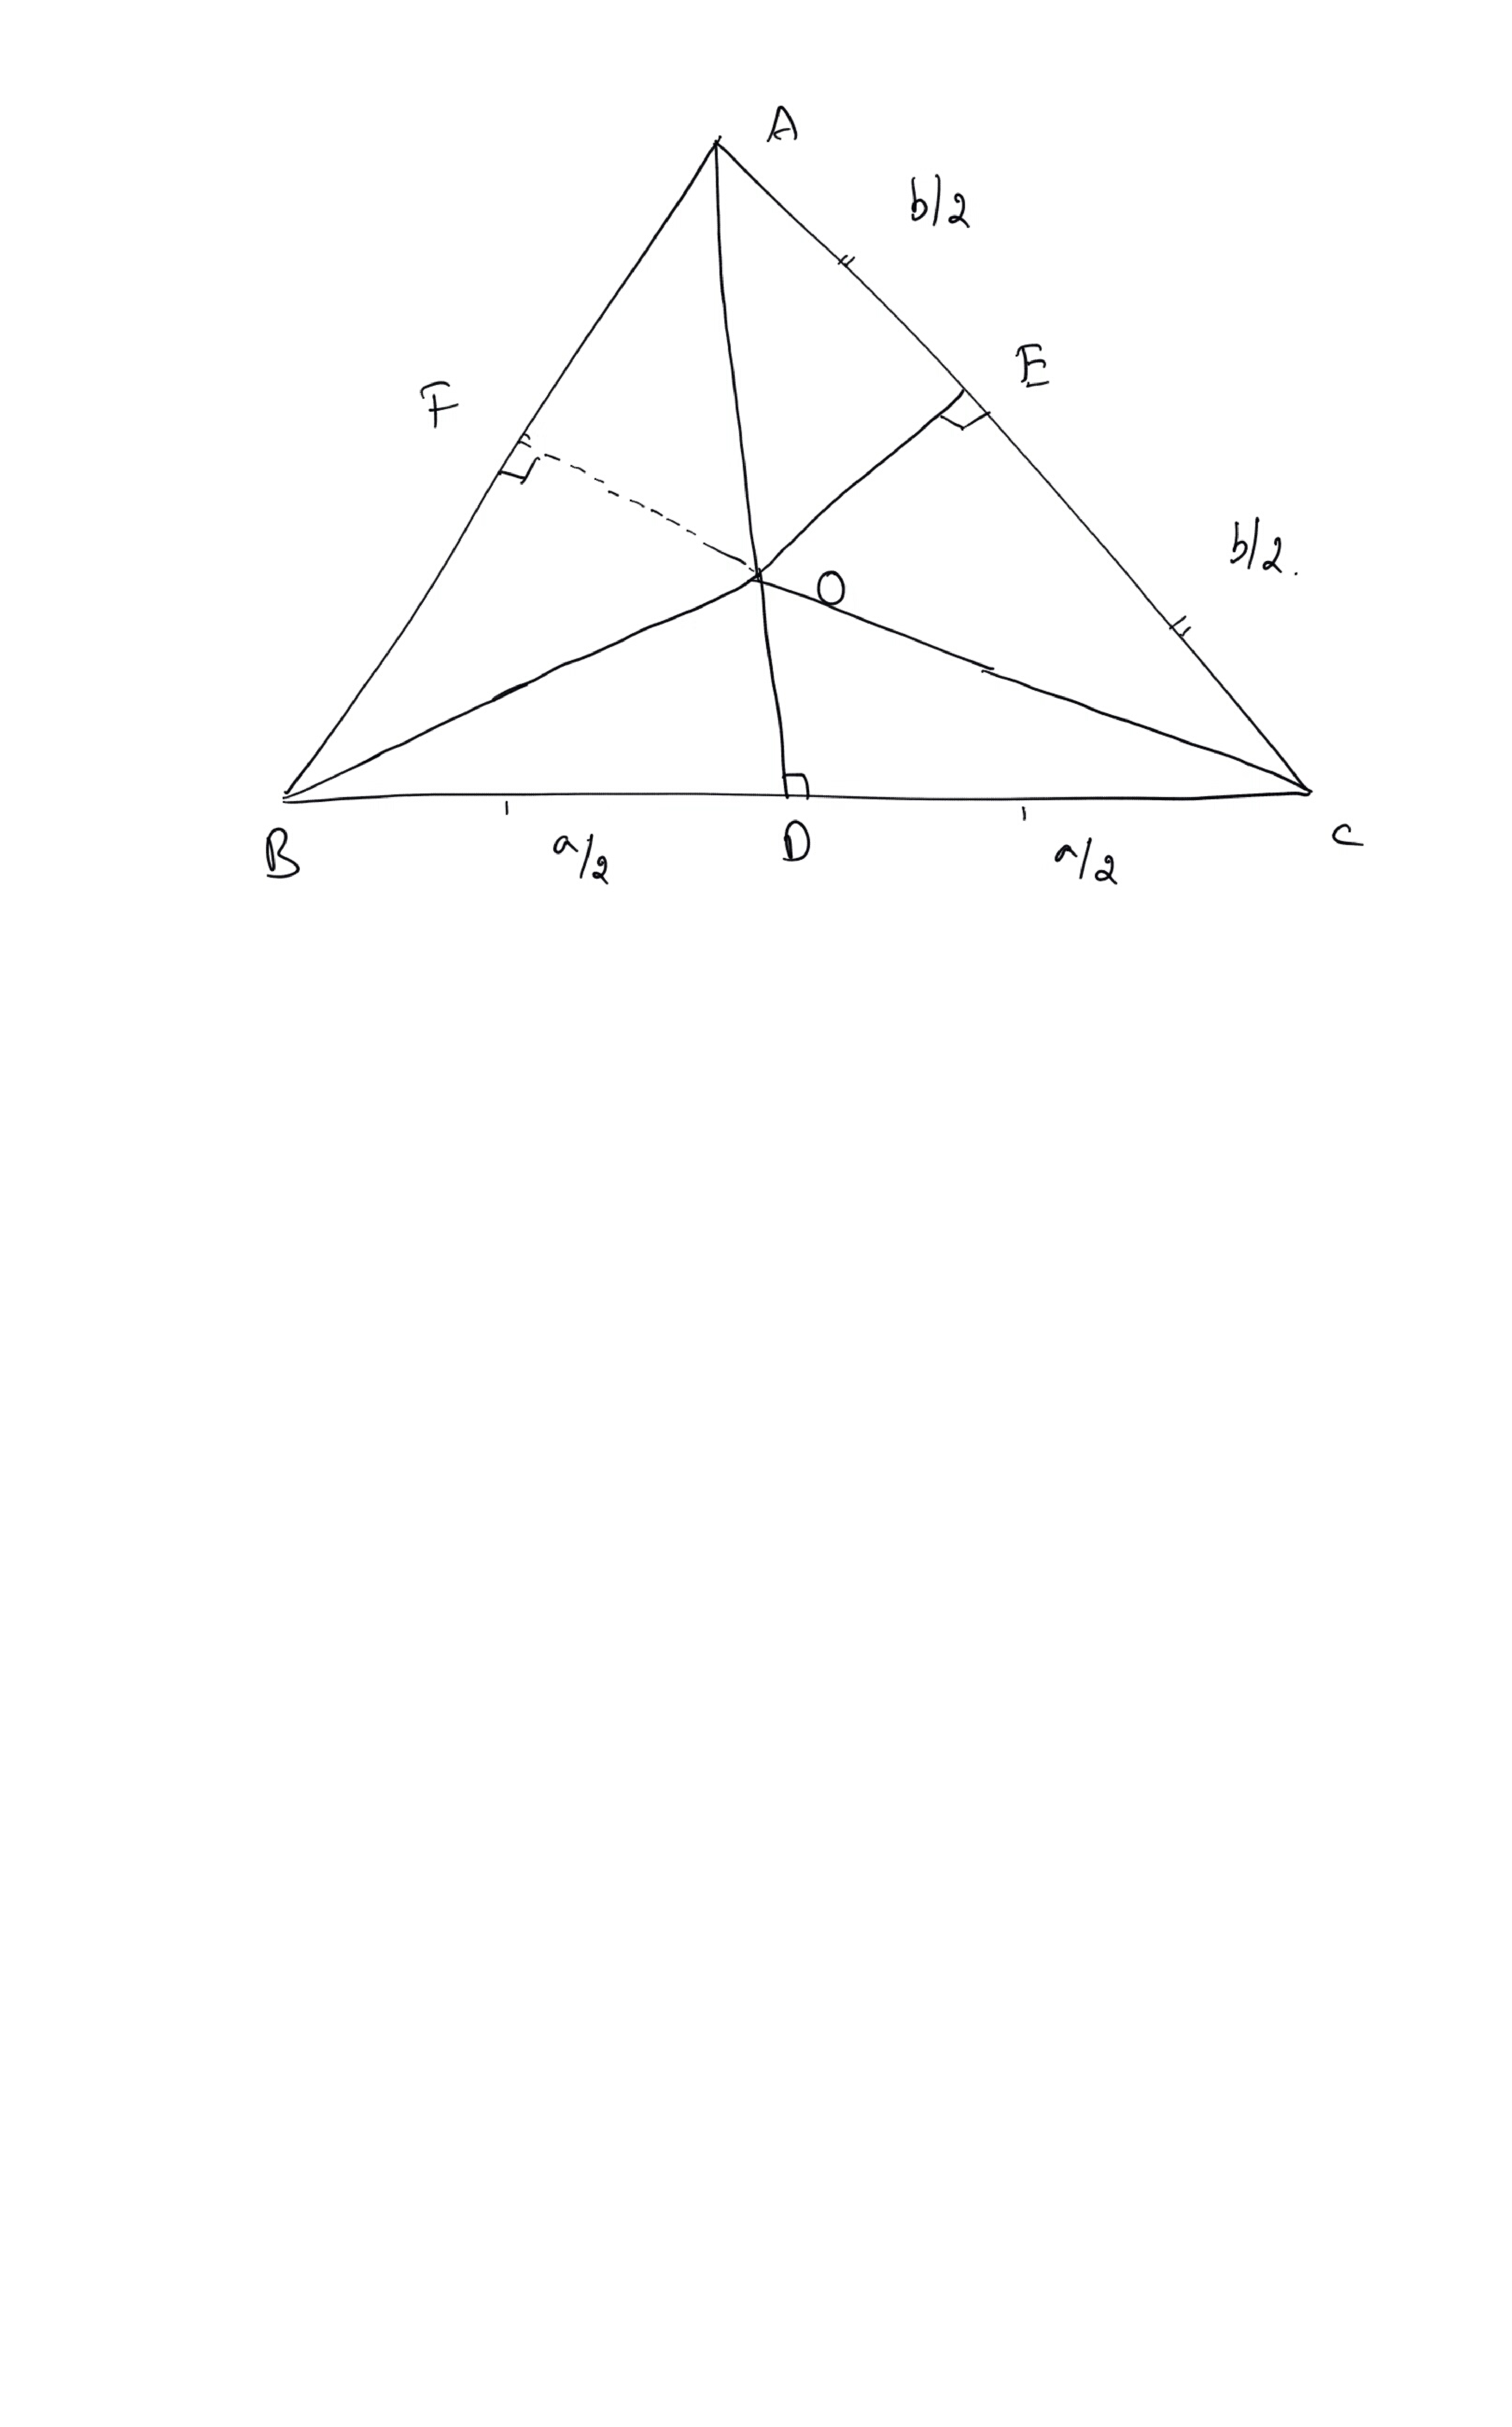
\includegraphics[width=\columnwidth]{./figs/ch3_perp_bisector}
		%\vspace*{-10cm}
%		\resizebox{\columnwidth}{!}{\documentclass{standalone}
\usepackage{tikz}
\usepackage{tkz-euclide}
\usetkzobj{all}
%\usepackage{amsmath}
\providecommand{\brak}[1]{\ensuremath{\left(#1\right)}}

\begin{document}
\begin{tikzpicture}
[scale=2,>=stealth,point/.style={draw,circle,fill = black,inner sep=0.5pt},]

\node (E) at (1.5, 1.5)[point,label=above :$E$] {};
\node (F) at (-1.5, 1.5)[point,label=above :$F$] {};
\node (A) at (0, 3)[point,label=above :$A$]{};
\node (B) at (-3, 0)[point,label=below left:$B$]{};
\node (C) at (3, 0)[point,label=below right:$C$]{};
\node (D) at (0,0)[point,label=below :$D$] {};
\node (O) at (0,1)[point,label=above right :$O$] {};


\draw (B)--(A);
\draw (A)--(C);
\draw (B)--(C);
\draw (B)--(E);
\draw (C)--(O);
\draw (A)--(D);
\draw [thick,dashed] (O) -- (F);

\node [above] at (1.7,1.7) {$b$};
\node [above] at (2.5,.75) {$b/2$};
\node [above] at (1,2.1) {$b/2$};
\node [above] at (-1.5,-0.3){$a/2$};
\node [above] at (1.5,-0.3){$a/2$};
\tkzMarkRightAngle[size=.16](B,F,O)
\tkzMarkRightAngle[size=.16](C,E,O)
\tkzMarkRightAngle[size=.2](A,D,C)
\draw   -- (4.3,1.7) node[midway] {$\parallel$};
\draw   -- (1.6,4.4) node[midway] {$\parallel$};

\end{tikzpicture}
\end{document}}
	\end{center}
	\caption{Perpendicular bisectors meet at a point}
	\label{ch3_perp_bisector}	
\end{figure}
%
\proof In $\Delta$s $ODB$ and $ODC$, using Budhayana's theorem,
%
\begin{equation}
\begin{split}
OB^2 &= OD^2 + BD^2 \\
OC^2 &= OD^2 + DC^2 
\end{split}
\end{equation}
%
Since $BD = DC = \frac{a}{2}$, $OB = OC$.  Similarly, it can be shown that $OA = OC$.  Thus, $OA=OB=OC$.
%
\begin{definition}
	In $\Delta AOB$, $OA = OB$.  Such a triangle is known as an isoceles triangle.
\end{definition}
%
\begin{problem}
	Show that $AF = BF$.
\end{problem}
\proof Trivial using Budhayana's theorem.  This shows that $OF$ is a perpendicular bisector of $AB$. 
{\em Conclusion:}  The perpendicular bisectors of a triangle meet at a point.
%
\subsection{Perpendiculars from Vertex to Opposite Side}
	%
	%
	In Fig. \ref{ch3_perp_triang}, $AD \perp BC$ and $BE \perp AC$. $CF$ passes through $O$ and meets
	$AB$ at $F$.  	
\begin{problem}
	Show that 
	\begin{align}
	OE = c \cos A \cot C
	\end{align}
\end{problem}
	\begin{figure}[!ht]
		\begin{center}
			
			%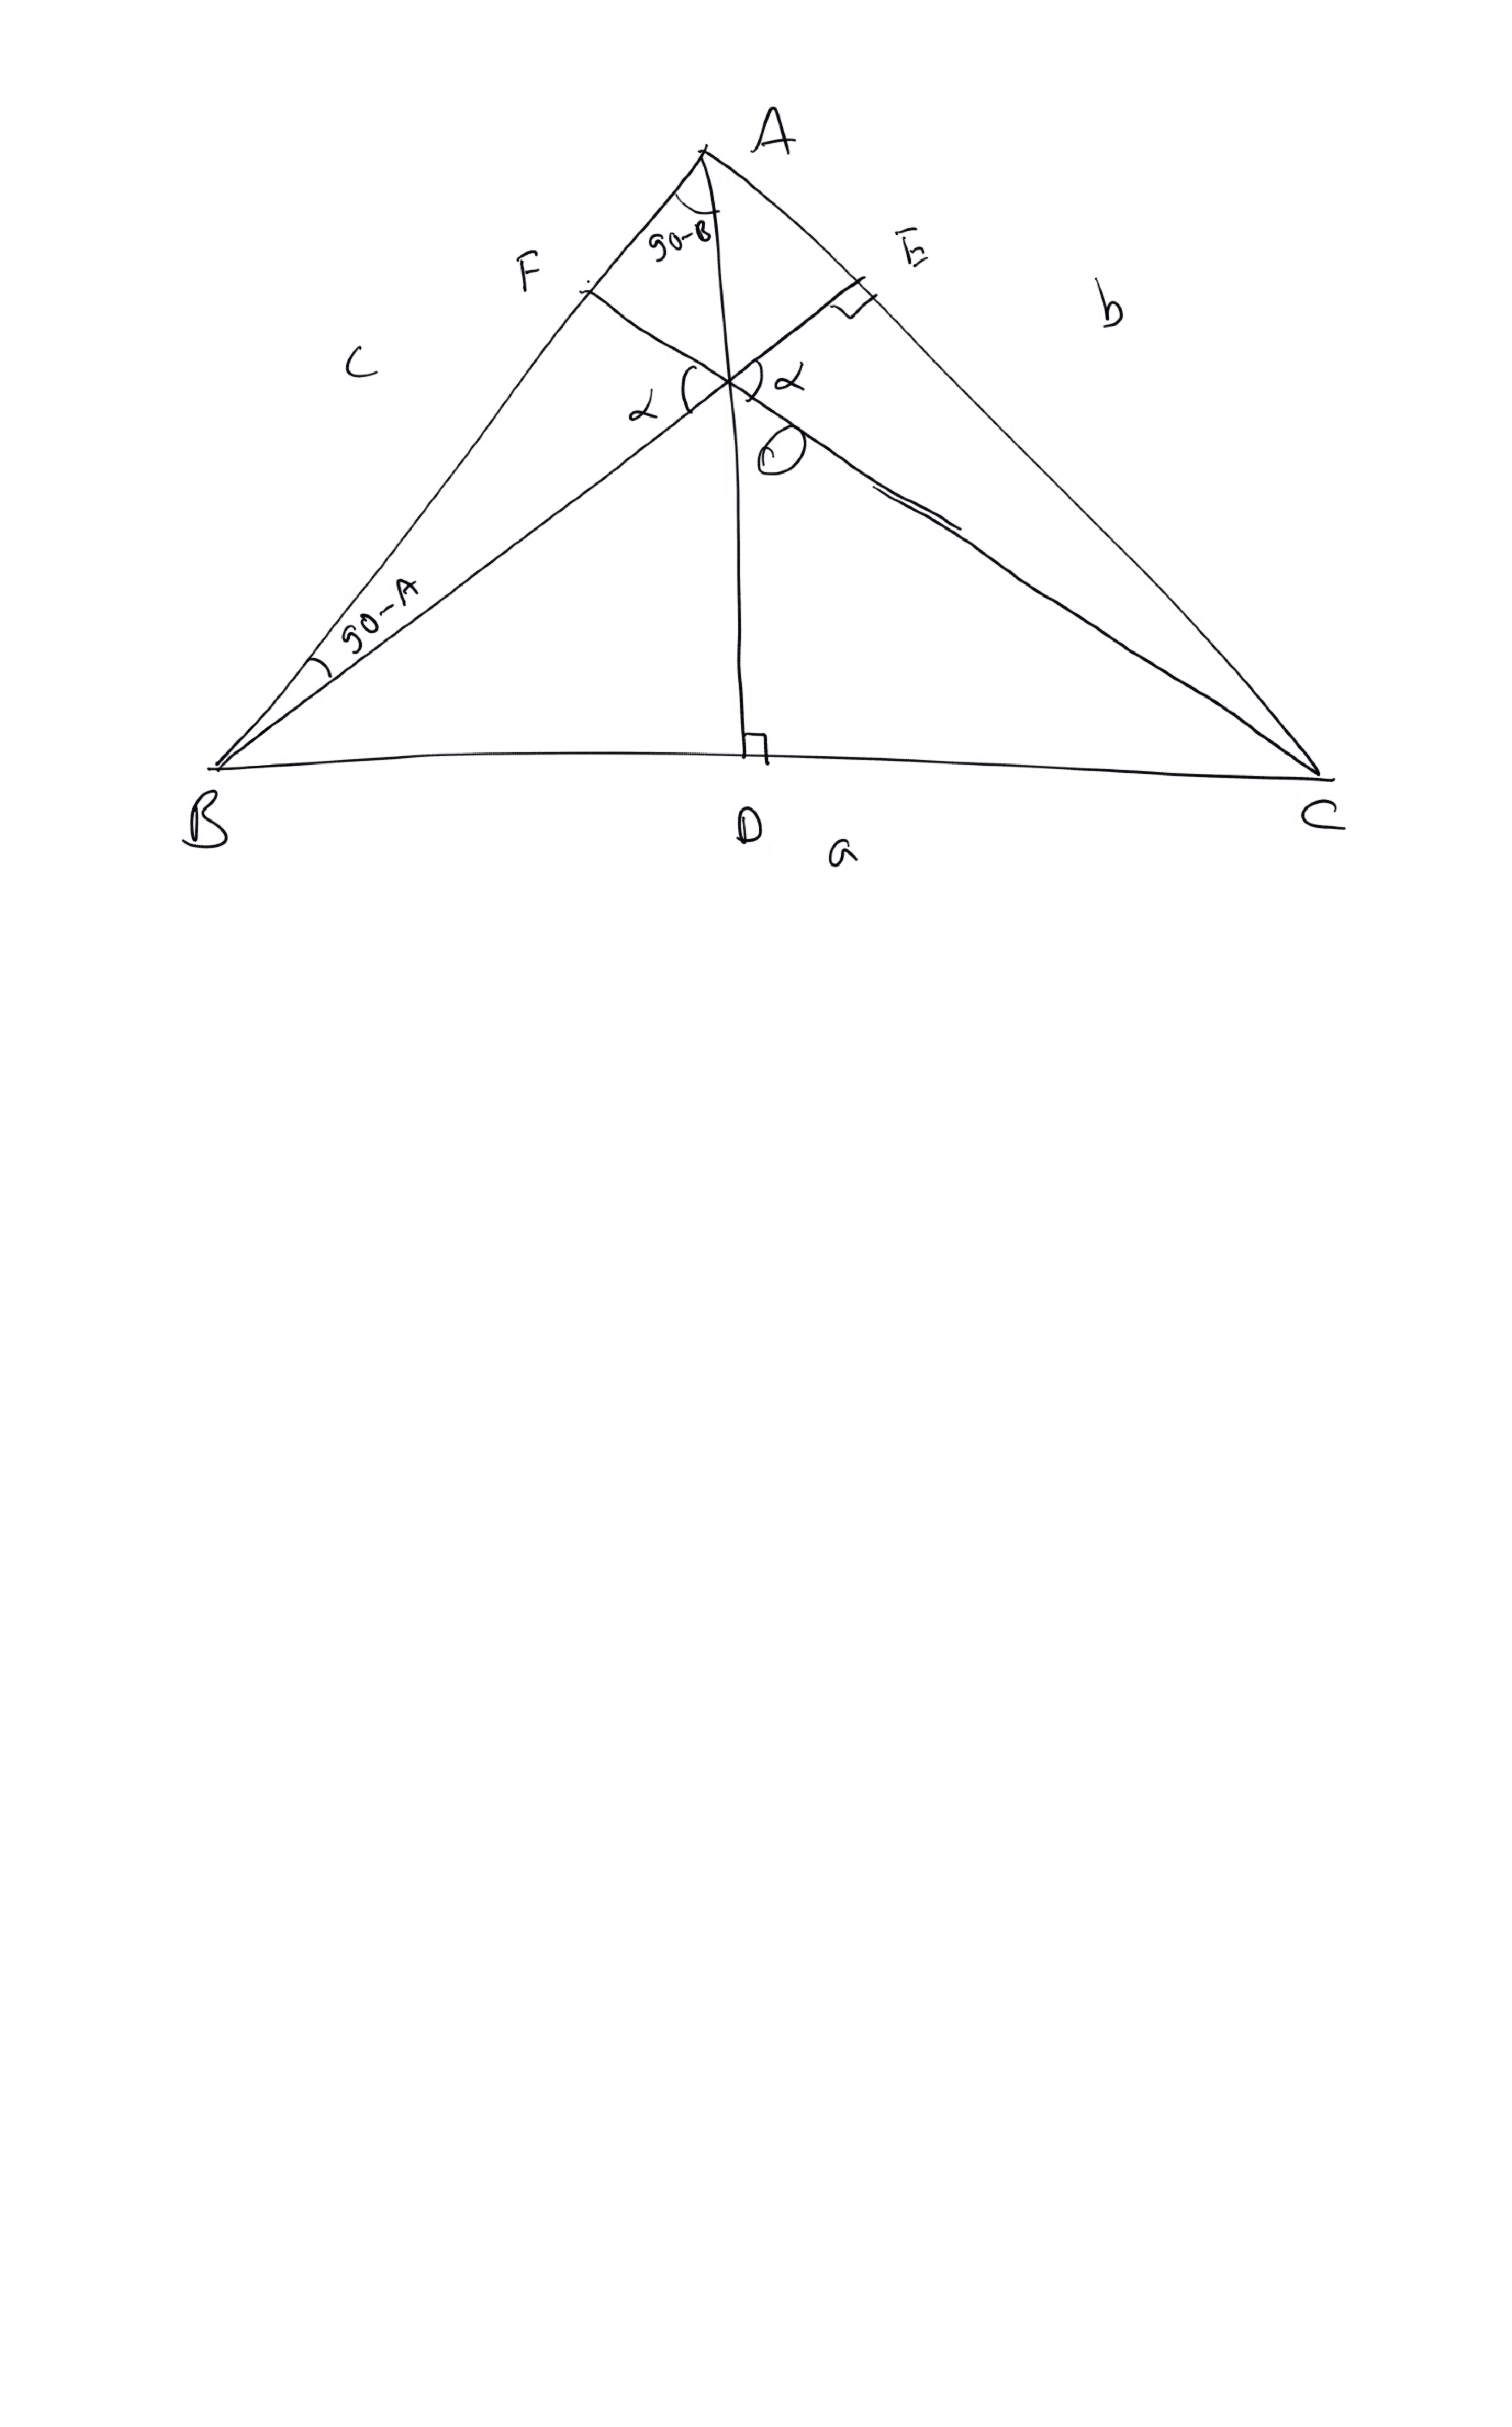
\includegraphics[width=\columnwidth]{./figs/ch3_perp_triang}
			%\vspace*{-10cm}
			\resizebox{\columnwidth}{!}{\begin{tikzpicture}
[scale=2,>=stealth,point/.style={draw,circle,fill = black,inner sep=0.5pt},]

\node (E) at (1.5, 1.5)[point,label=above :$E$] {};
\node (F) at (-1.5, 1.5)[point,label=above :$F$] {};
\node (A) at (0, 3)[point,label=above :$A$]{};
\node (B) at (-3, 0)[point,label=below left:$B$]{};
\node (C) at (3, 0)[point,label=below right:$C$]{};
\node (O) at (0,1)[point,label=above right :$O$] {};
\node (D) at (0,0)[point,label=below :$D$] {};


\draw (B)--(A);
\draw (A)--(C);
\draw (B)--(E);
\draw (C)--(F);
\draw (B)--(C);
\draw (A)--(D);

\node [below] at (0,-0.3) {$a$};
\node [above] at (-1.7,1.7) {$c$};
\node [above] at (1.7,1.7) {$b$};
\node [above] at (1,1.3) {$p$};
\node [above] at (-1,1.3) {$q$};
\node [above] at (-2.3,0.24){\rotatebox{45}{$90-A$}};
\node [above] at (-0.4,2.1) {\rotatebox{45}{$90-B$}};
\node [above] at (0.4,2.1) {\rotatebox{-45}{$90-C$}};

\tkzMarkAngle[size=.3](F,O,B);
\tkzMarkAngle[size=.3](C,O,E);
\tkzMarkAngle[size=.4](O,B,F);
\tkzMarkAngle[size=.2](F,A,O);
\tkzMarkAngle[size=.3](O,A,E);
\draw (-0.5,1) node{$\alpha$};
\draw (0.5,1) node{$\alpha$};

\end{tikzpicture}
}
		\end{center}
		\caption{Perpendiculars from vertex to opposite side meet at a point}
		\label{ch3_perp_triang}	
	\end{figure}
%
\proof In $\Delta$ s $AEB$ and $AEO$,
%
\begin{align}
AE &= c \cos A \\
OE &= AE \tan \brak{90^{\degree} - C} \brak{\because ADC \text{ is right angled}} \\
&= AE \cot C
\end{align}
%
From both the above, we get the desired result.
%
\begin{problem}
	Show that $\alpha = A$.
\end{problem}
\proof In $\Delta OEC$,
%
\begin{equation}
CE = a \cos C \brak{\because BEC \text{ is right angled}}
\end{equation}
%
Hence,
%
\begin{equation}
\begin{split}
\tan \alpha &= \frac{CE}{OE} \\
&=  \frac{a \cos C}{c \cos A \cot C} \\
&=  \frac{a \cos C \sin C}{c \cos A \cos C} \\
&= \frac{a \sin C}{c \cos A } \\
&= \frac{c \sin A}{c \cos A } \brak{\because \frac{a}{\sin A} = \frac{c}{\sin C}}\\
&= \tan A\\
\Rightarrow \alpha = A
\end{split}
\end{equation}
%
\begin{problem}
	Show that $CF \perp AB$
\end{problem}
\proof Consider triangle OFB and the result of the previous problem.  $\because$ the sum of the angles of a triangle is $180^{\degree}$, $\angle CFB = 90^{\degree}$.
{\em Conclusion: The perperdiculars from the vertex of a triangle to the opposite side meet at a point.}